\documentclass[11pt, oneside]{scrartcl}   	% use "amsart" instead of "article" for AMSLaTeX format
\usepackage[portrait]{geometry}               		% See geometry.pdf to learn the layout options. There are lots.
\geometry{a4paper}                   		% ... or a4paper or a5paper or ... 
%\geometry{landscape}                		% Activate for rotated page geometry
%\usepackage[parfill]{parskip}    		% Activate to begin paragraphs with an empty line rather than an indent
\usepackage{graphicx}				% Use pdf, png, jpg, or eps with pdflatex; use eps in DVI mode
% TeX will automatically convert eps --> pdf in pdflatex		
\usepackage{amssymb}
% \usepackage{wallpaper}
\usepackage{listings}
\usepackage{color}

\definecolor{mygreen}{rgb}{0,0.6,0}
\definecolor{mygray}{rgb}{0.5,0.5,0.5}
\definecolor{mymauve}{rgb}{0.58,0,0.82}

\lstset{ 
	backgroundcolor=\color{white},   % choose the background color; you must add \usepackage{color} or \usepackage{xcolor}; should come as last argument
	basicstyle=\footnotesize,        % the size of the fonts that are used for the code
	breakatwhitespace=false,         % sets if automatic breaks should only happen at whitespace
	breaklines=true,                 % sets automatic line breaking
	captionpos=b,                    % sets the caption-position to bottom
	commentstyle=\color{mygreen},    % comment style
	deletekeywords={...},            % if you want to delete keywords from the given language
	escapeinside={\%*}{*)},          % if you want to add LaTeX within your code
	extendedchars=true,              % lets you use non-ASCII characters; for 8-bits encodings only, does not work with UTF-8
	firstnumber=1000,                % start line enumeration with line 1000
	frame=single,	                   % adds a frame around the code
	keepspaces=true,                 % keeps spaces in text, useful for keeping indentation of code (possibly needs columns=flexible)
	keywordstyle=\color{blue},       % keyword style
	language=Octave,                 % the language of the code
	morekeywords={*,...},            % if you want to add more keywords to the set
	numbers=left,                    % where to put the line-numbers; possible values are (none, left, right)
	numbersep=5pt,                   % how far the line-numbers are from the code
	numberstyle=\tiny\color{mygray}, % the style that is used for the line-numbers
	rulecolor=\color{black},         % if not set, the frame-color may be changed on line-breaks within not-black text (e.g. comments (green here))
	showspaces=false,                % show spaces everywhere adding particular underscores; it overrides 'showstringspaces'
	showstringspaces=false,          % underline spaces within strings only
	showtabs=false,                  % show tabs within strings adding particular underscores
	stepnumber=2,                    % the step between two line-numbers. If it's 1, each line will be numbered
	stringstyle=\color{mymauve},     % string literal style
	tabsize=2,	                   % sets default tabsize to 2 spaces
	title=\lstname                   % show the filename of files included with \lstinputlisting; also try caption instead of title
}

\usepackage[headsepline]{scrlayer-scrpage}
\pagestyle{scrheadings}
\clearpairofpagestyles
% \ohead{\textsf{Section \thesection}}  % \thesection
\ihead{\textsf{Audio Signal Generator}}
\ohead{\headmark}
% \chead[\pagemark]{Page \pagemark}
\automark[subsection]{section}
% \chead{\textsf{Page \thepage}}
\cfoot[\pagemark]{Page \pagemark}

\setlength{\parindent}{0pt}

\usepackage{eso-pic}


\begin{document}

	%%%%%%%%%%%%%%%%%%%%%%%%%%%%%%%%%%%%%%%%%%%%%%%%%%%%%%%%%%%%%%%
	\begingroup
	\thispagestyle{empty}
	\centering
	% \AddToShipoutPicture*{\put(0,400){\includegraphics[scale=1.0]{Pisound.jpg}}} % Image background
	% \AddToShipoutPicture*{\put(60,60){\includegraphics[scale=1.0]{DualPowerSupply.png}}} % Image background
	\AddToShipoutPicture*{\put(120,500){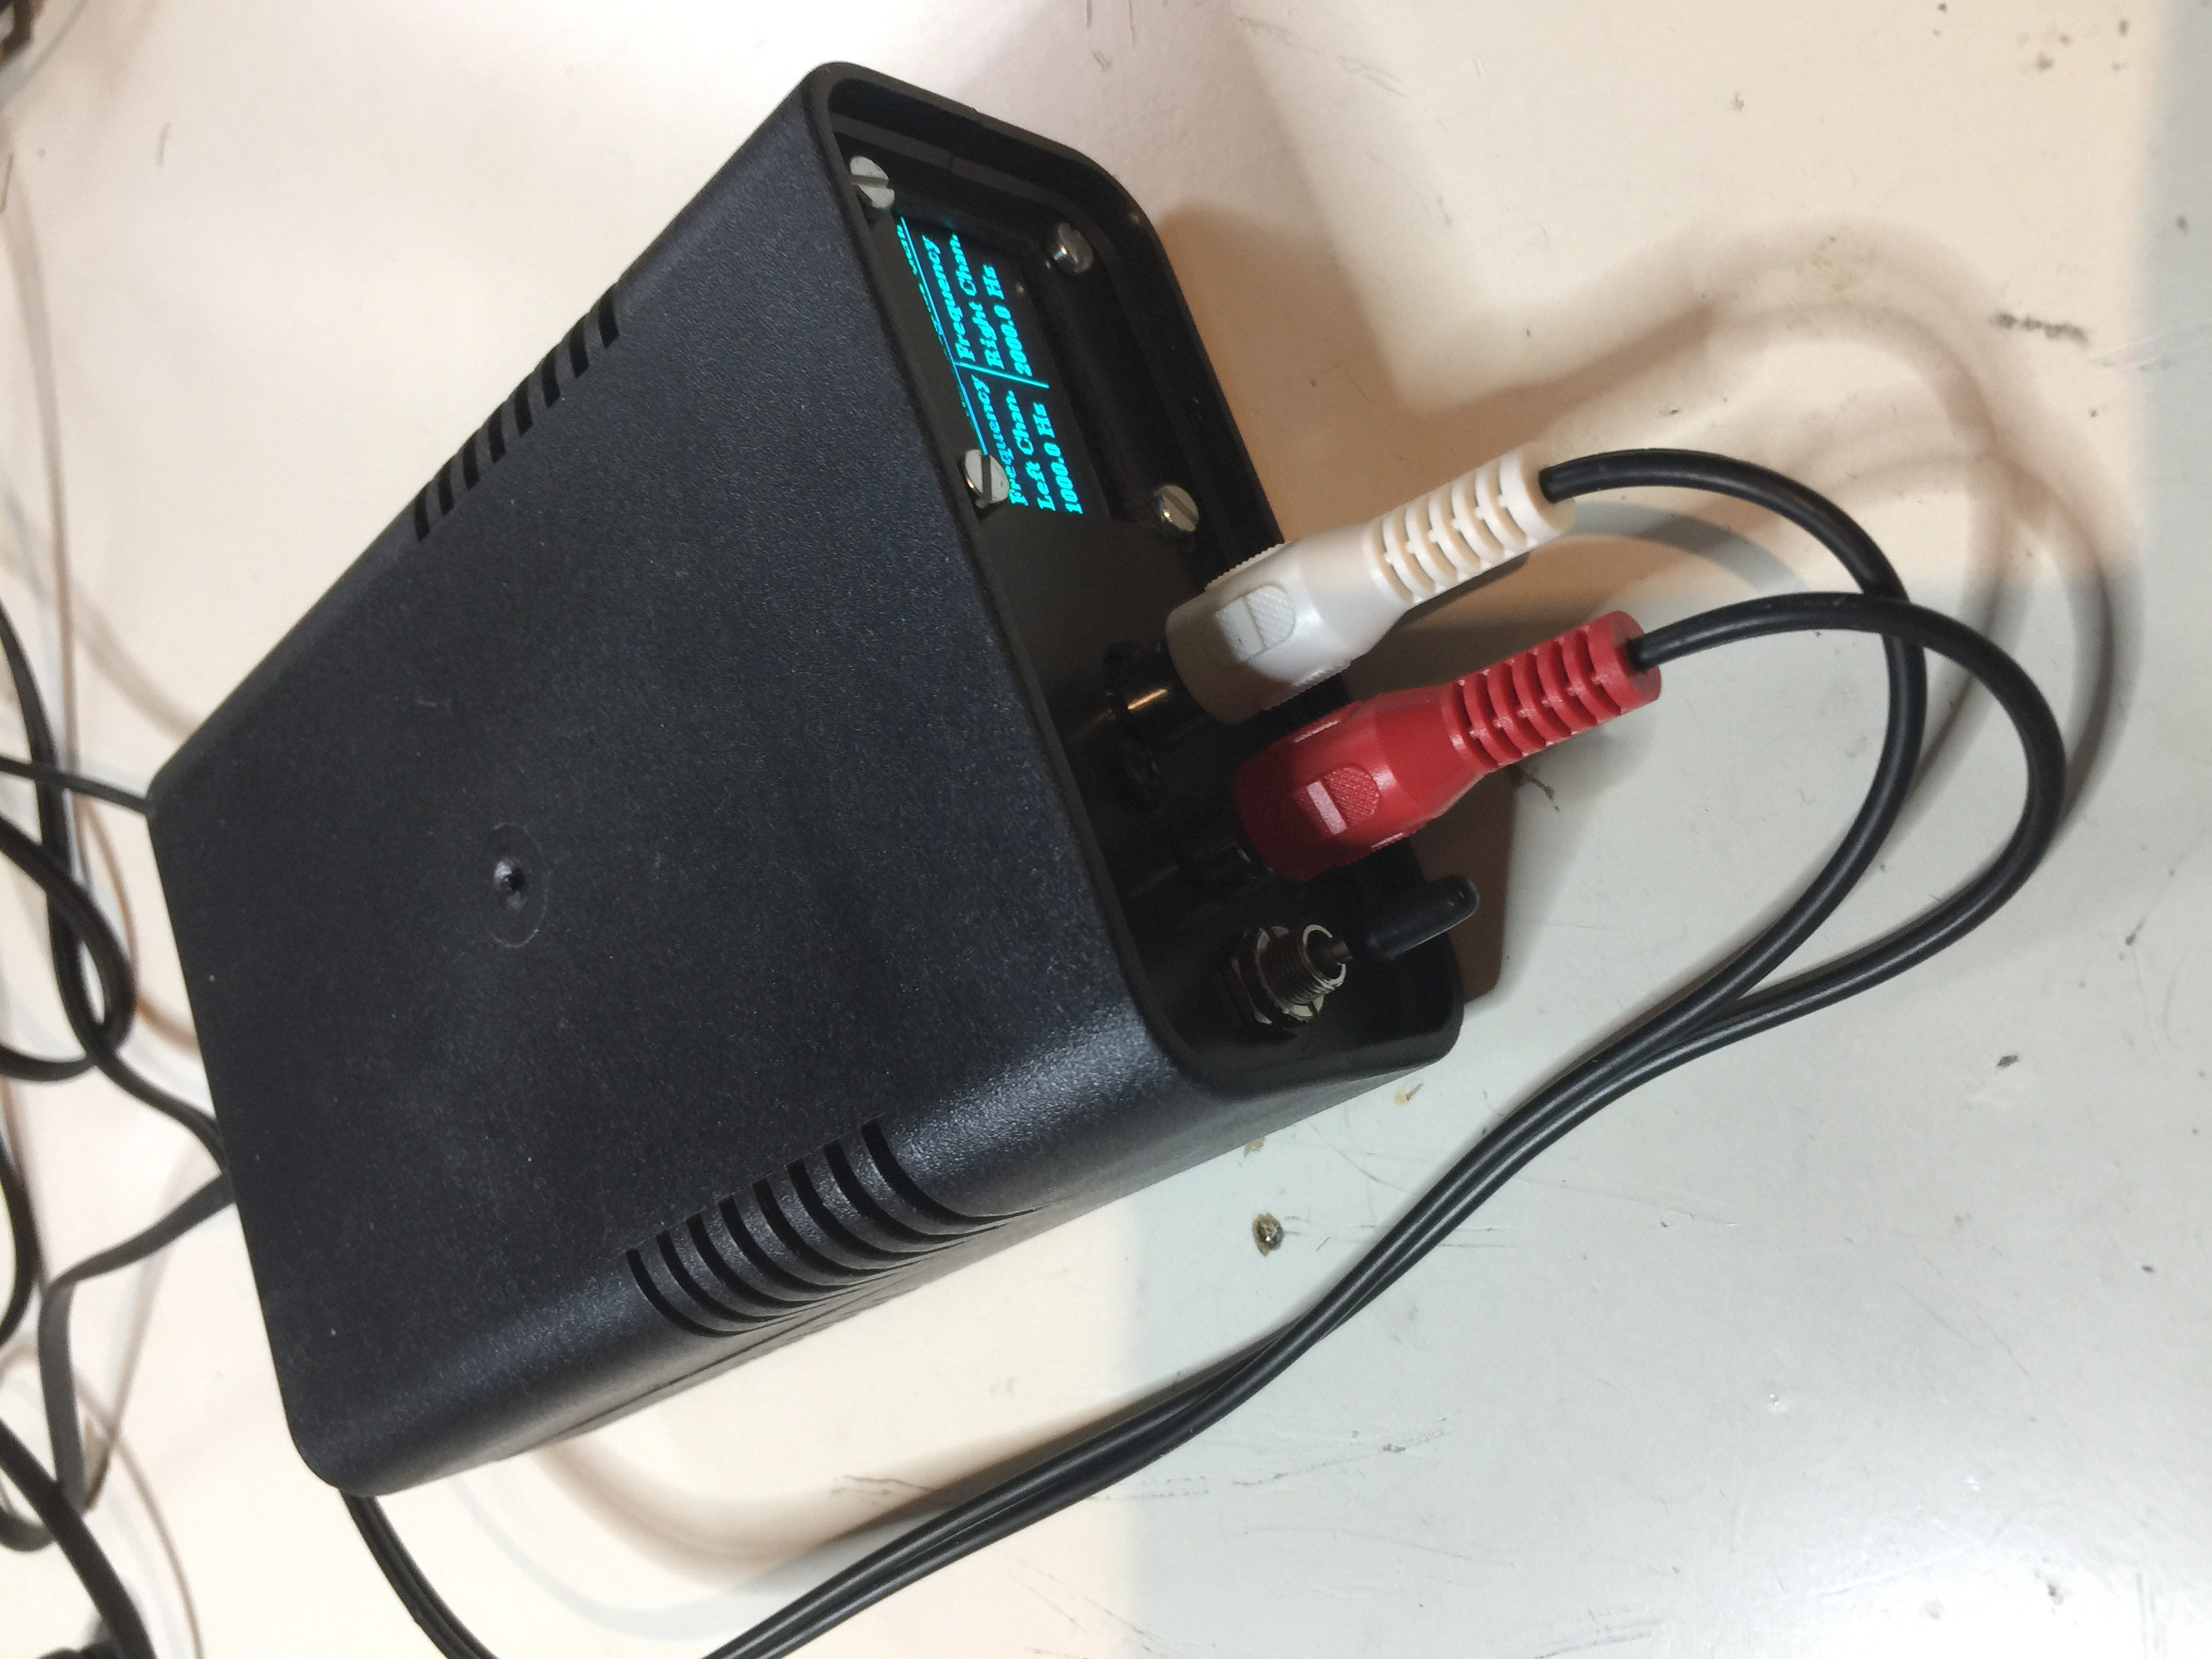
\includegraphics[scale=0.15,angle=-90 ]{AudioSignalGeneratorTopFrontViewClosed.jpeg}}} % Image background
	
	\par\normalfont\fontsize{30}{30}\sffamily\selectfont
	\vspace*{-0.5cm}
	{\color{black}
		\textbf{\Huge Stereo Audio Signal Generator}\\
		\vspace*{1.5cm}
		{\textbf\huge Documentation}\par % Book title
		\vspace*{0.5cm}
		{\textbf \huge by Dr. Markus Reinhardt}\par % Author name
		\vspace*{1.5cm}
		{\textbf \huge \today}\par
	}
	\endgroup
	\vfill
	
	% \maketitle
	
	\newpage
	\thispagestyle{empty}
	\tableofcontents
	
	\thispagestyle{empty}
	\listoffigures
	% \listoftables
	
	\newpage
	\pagestyle{scrheadings}
	
\section{Block diagram}                         
The block diagram (equal to the schematics) of the \textbf{Stereo Audio Signal Generator} is shown in figure \ref{fig:toplevelfunctionalblock}:
\begin{figure}[tbph]
	\centering
	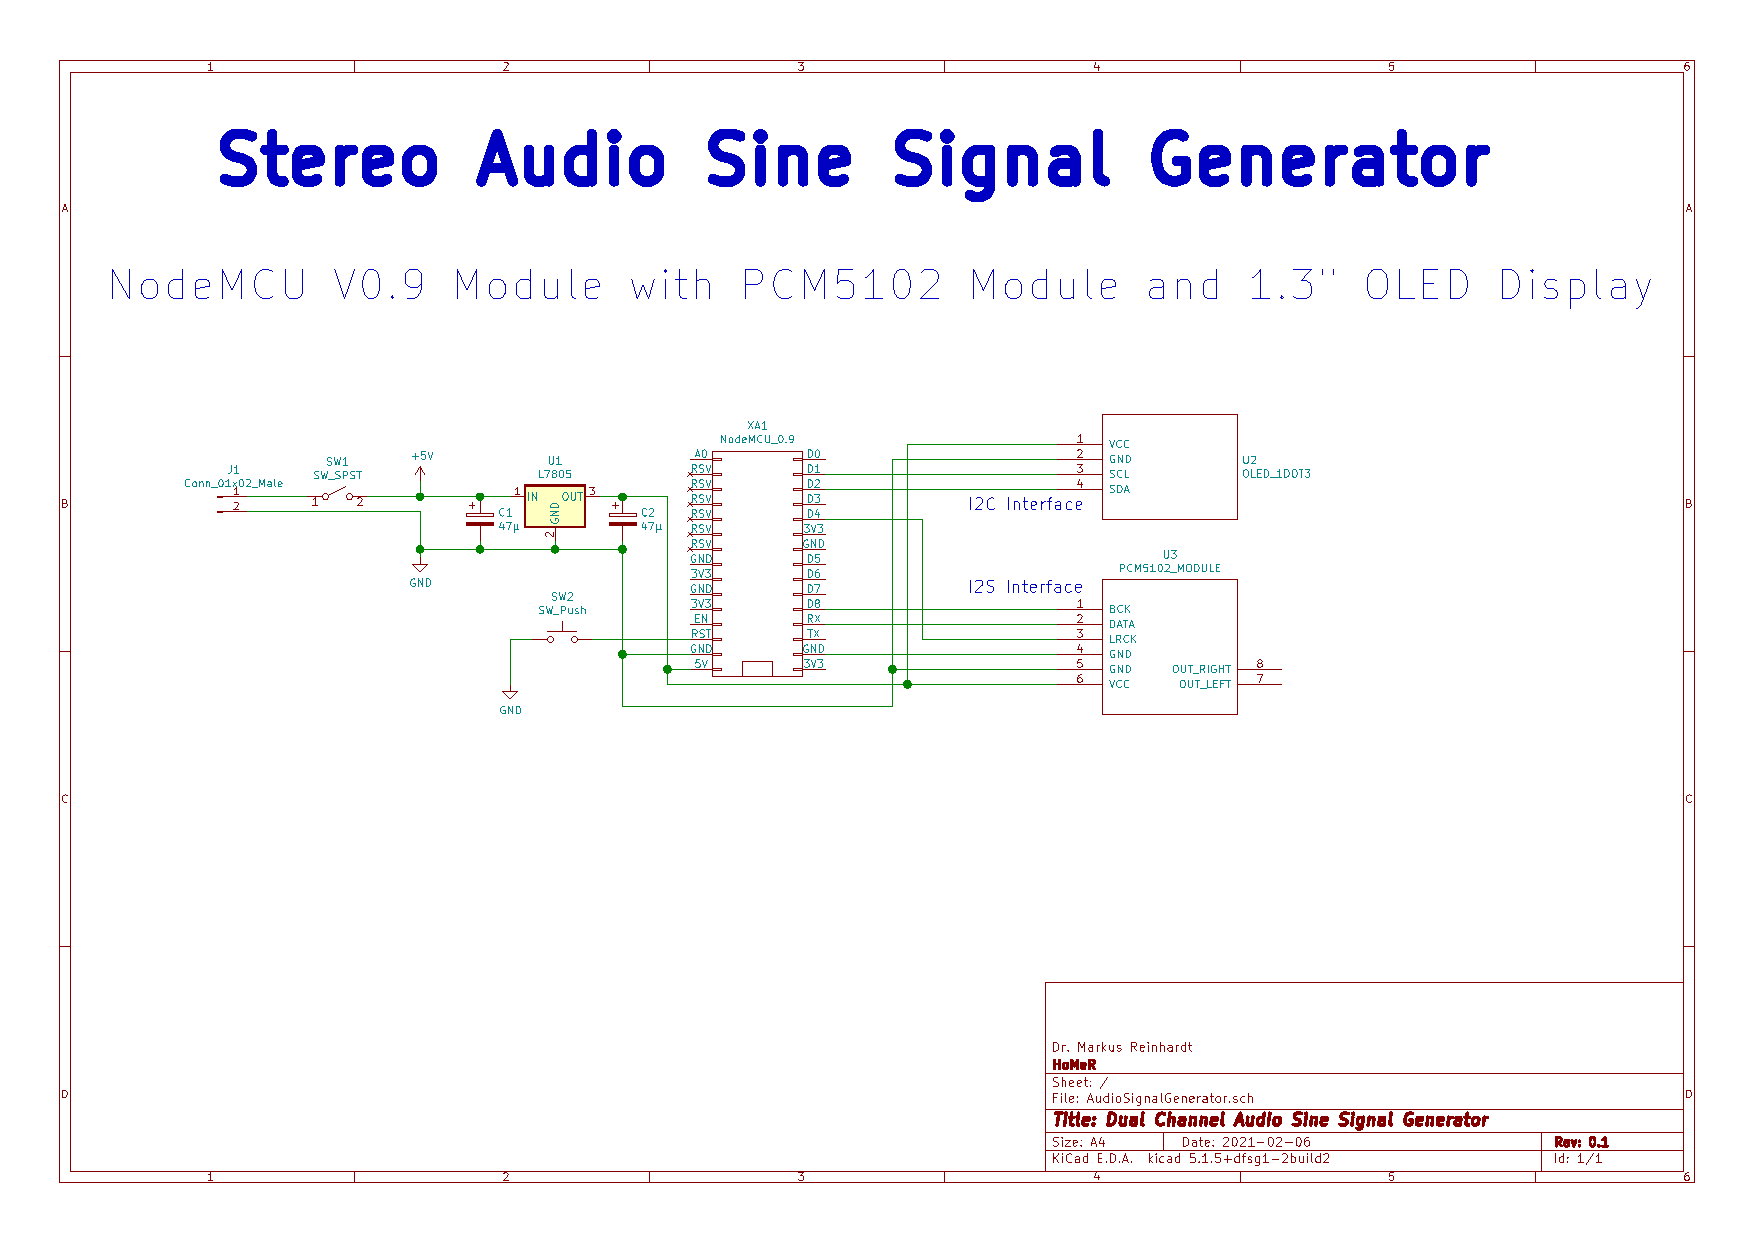
\includegraphics[width=\linewidth]{AudioSignalGeneratorSchematics.pdf}
	\caption[Stereo Audio Signal Generator top level block diagram]{Stereo Audio Signal Generator top level block diagram}
	\label{fig:toplevelfunctionalblock}
\end{figure}
The device consists of a NodeMCU module (V0.9) feeding a DAC module with a DAC of type PCM5102 via the I2S interface, a 1.3" OLED display fed from the controller via the I2C interface and a power supply with an external SMPS module connected to the
5V voltage regulator of type LM7805.
\newpage

\section{Hardware description}
\subsection{Casing}
The Stereo Audio Signal Generator is housed in a standard black plastic case, see the following picture:
\begin{figure}[tbph]
	\centering
	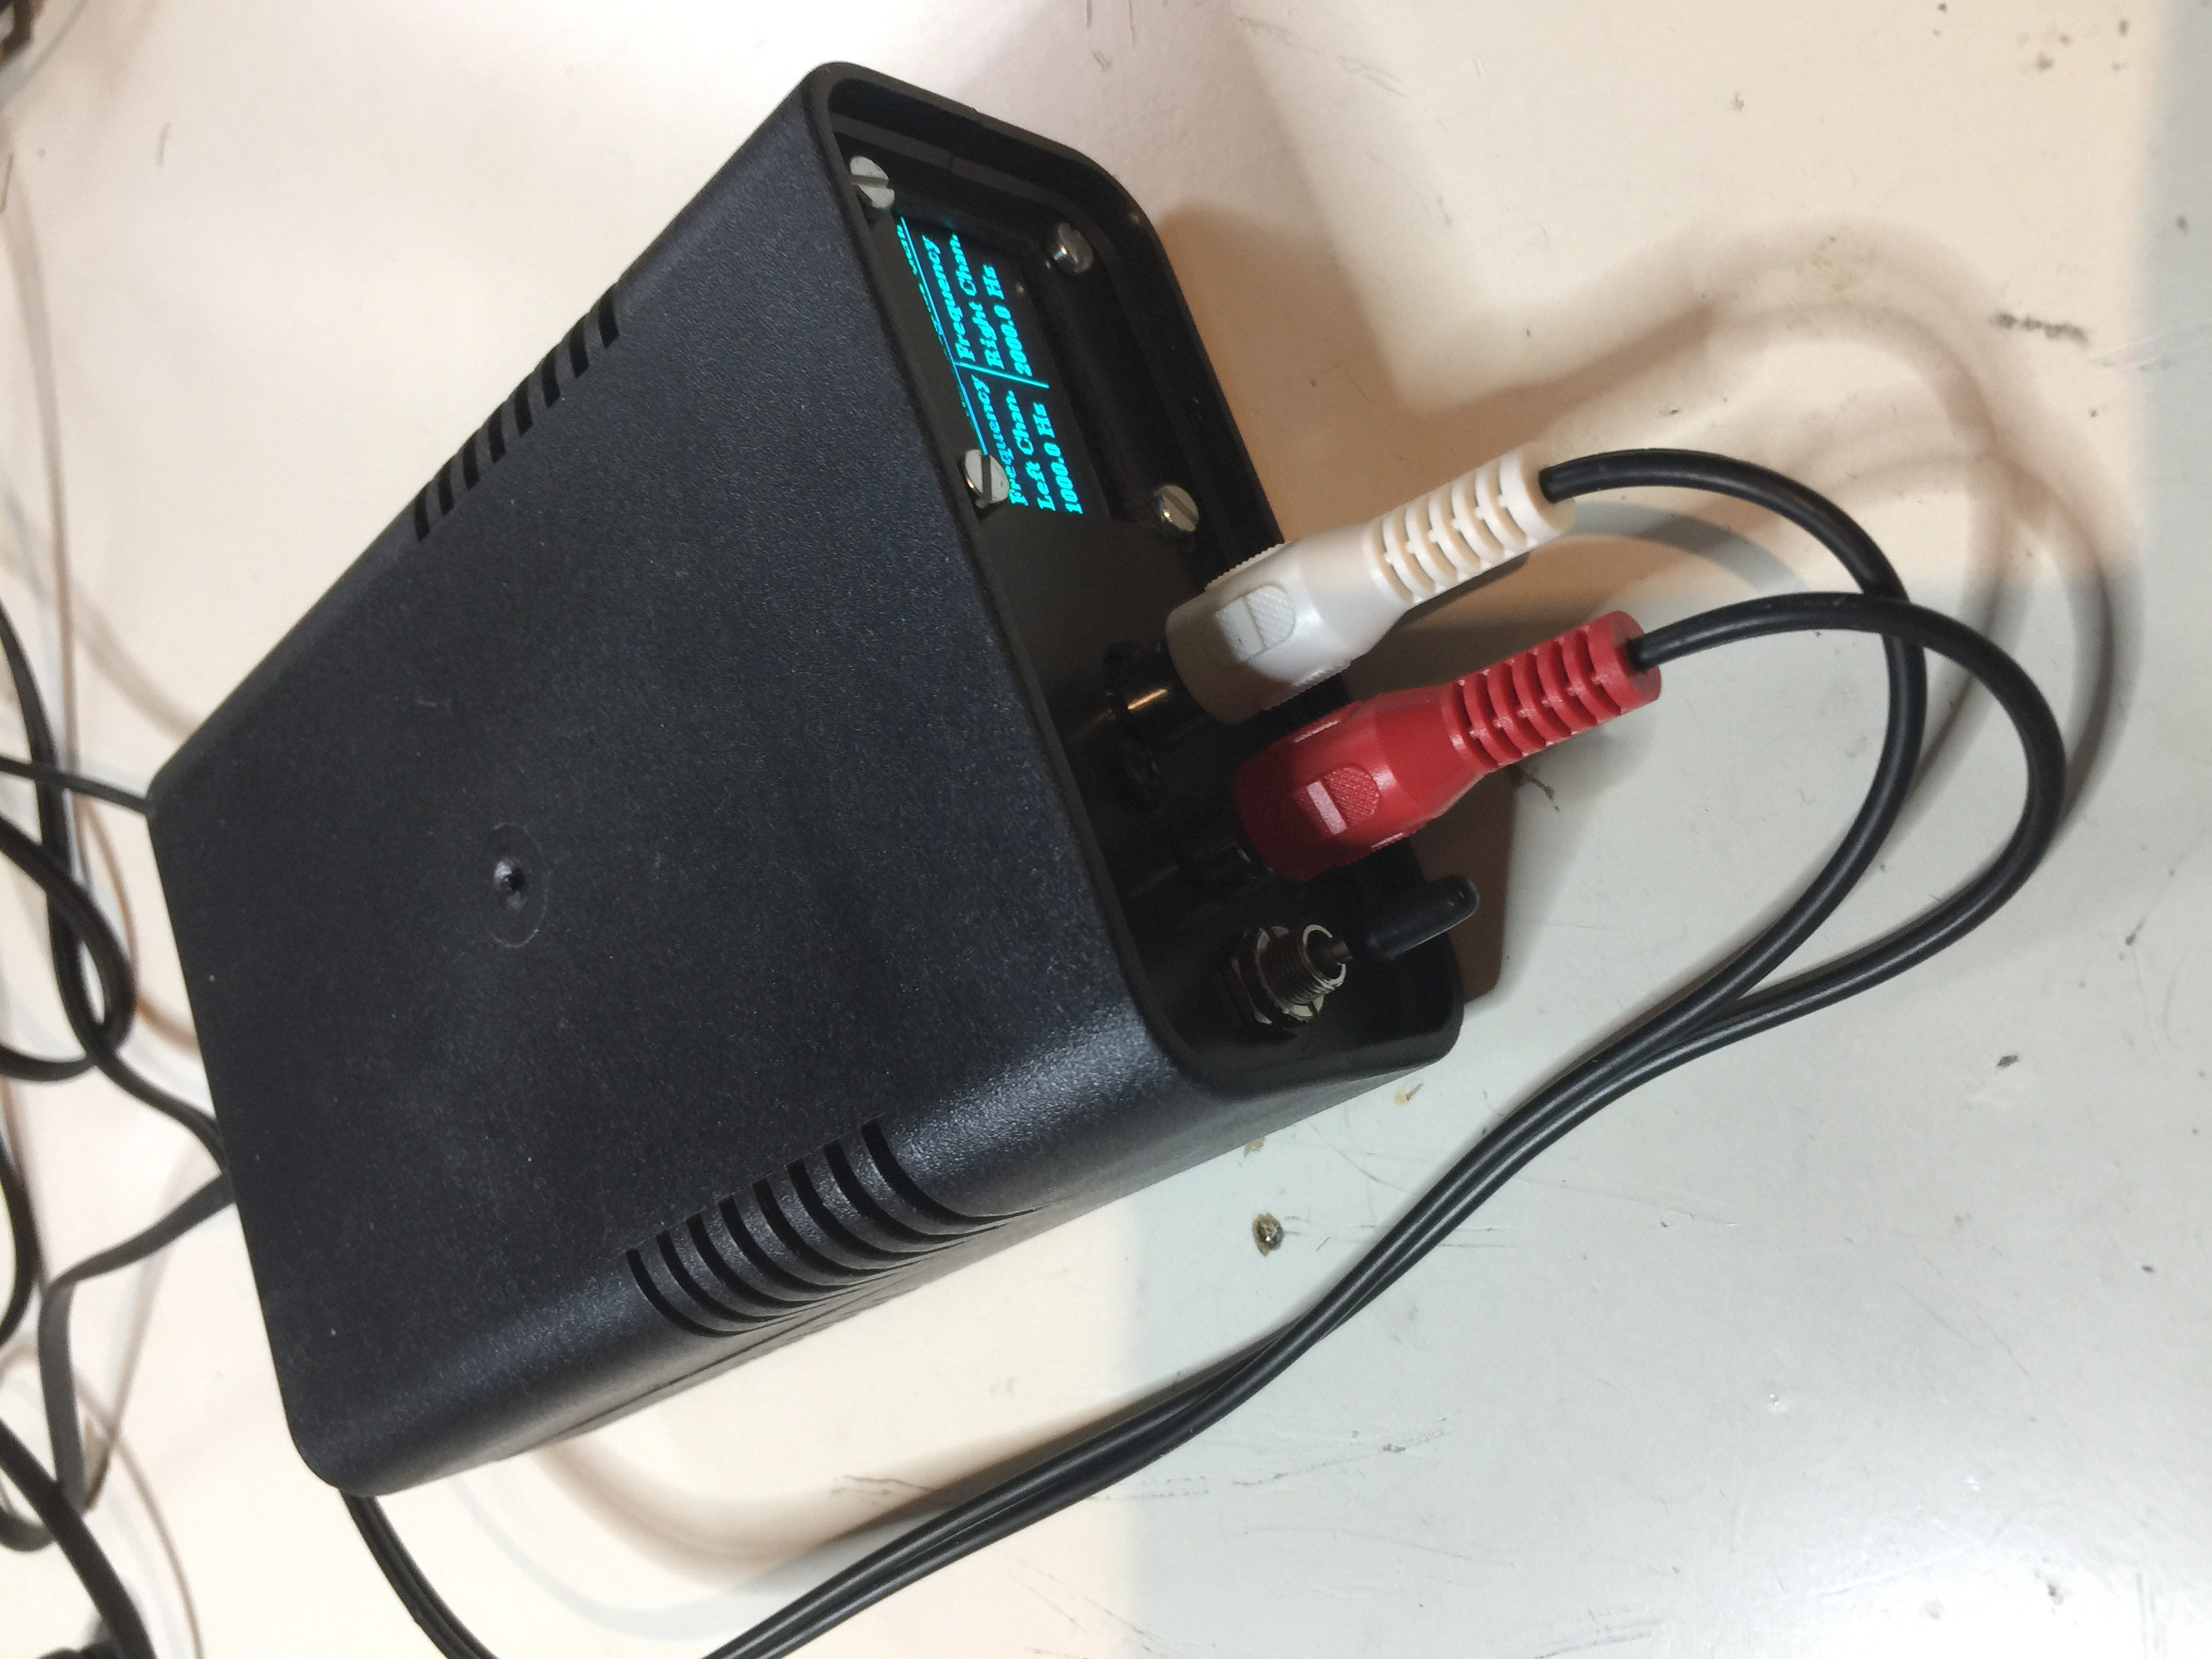
\includegraphics[width=\linewidth, angle=-90]{AudioSignalGeneratorTopFrontViewClosed.jpeg}
	\caption[Audio Signal Generator top level block diagram]{Audio Signal Generator top level block diagram}
	\label{fig:casing}
\end{figure}
\newpage

\subsection{Mechanical assembly}
The mechanical assembly inside the case is shown in figure \ref{fig:mechanics}
\begin{figure}[tbph]
	\centering
	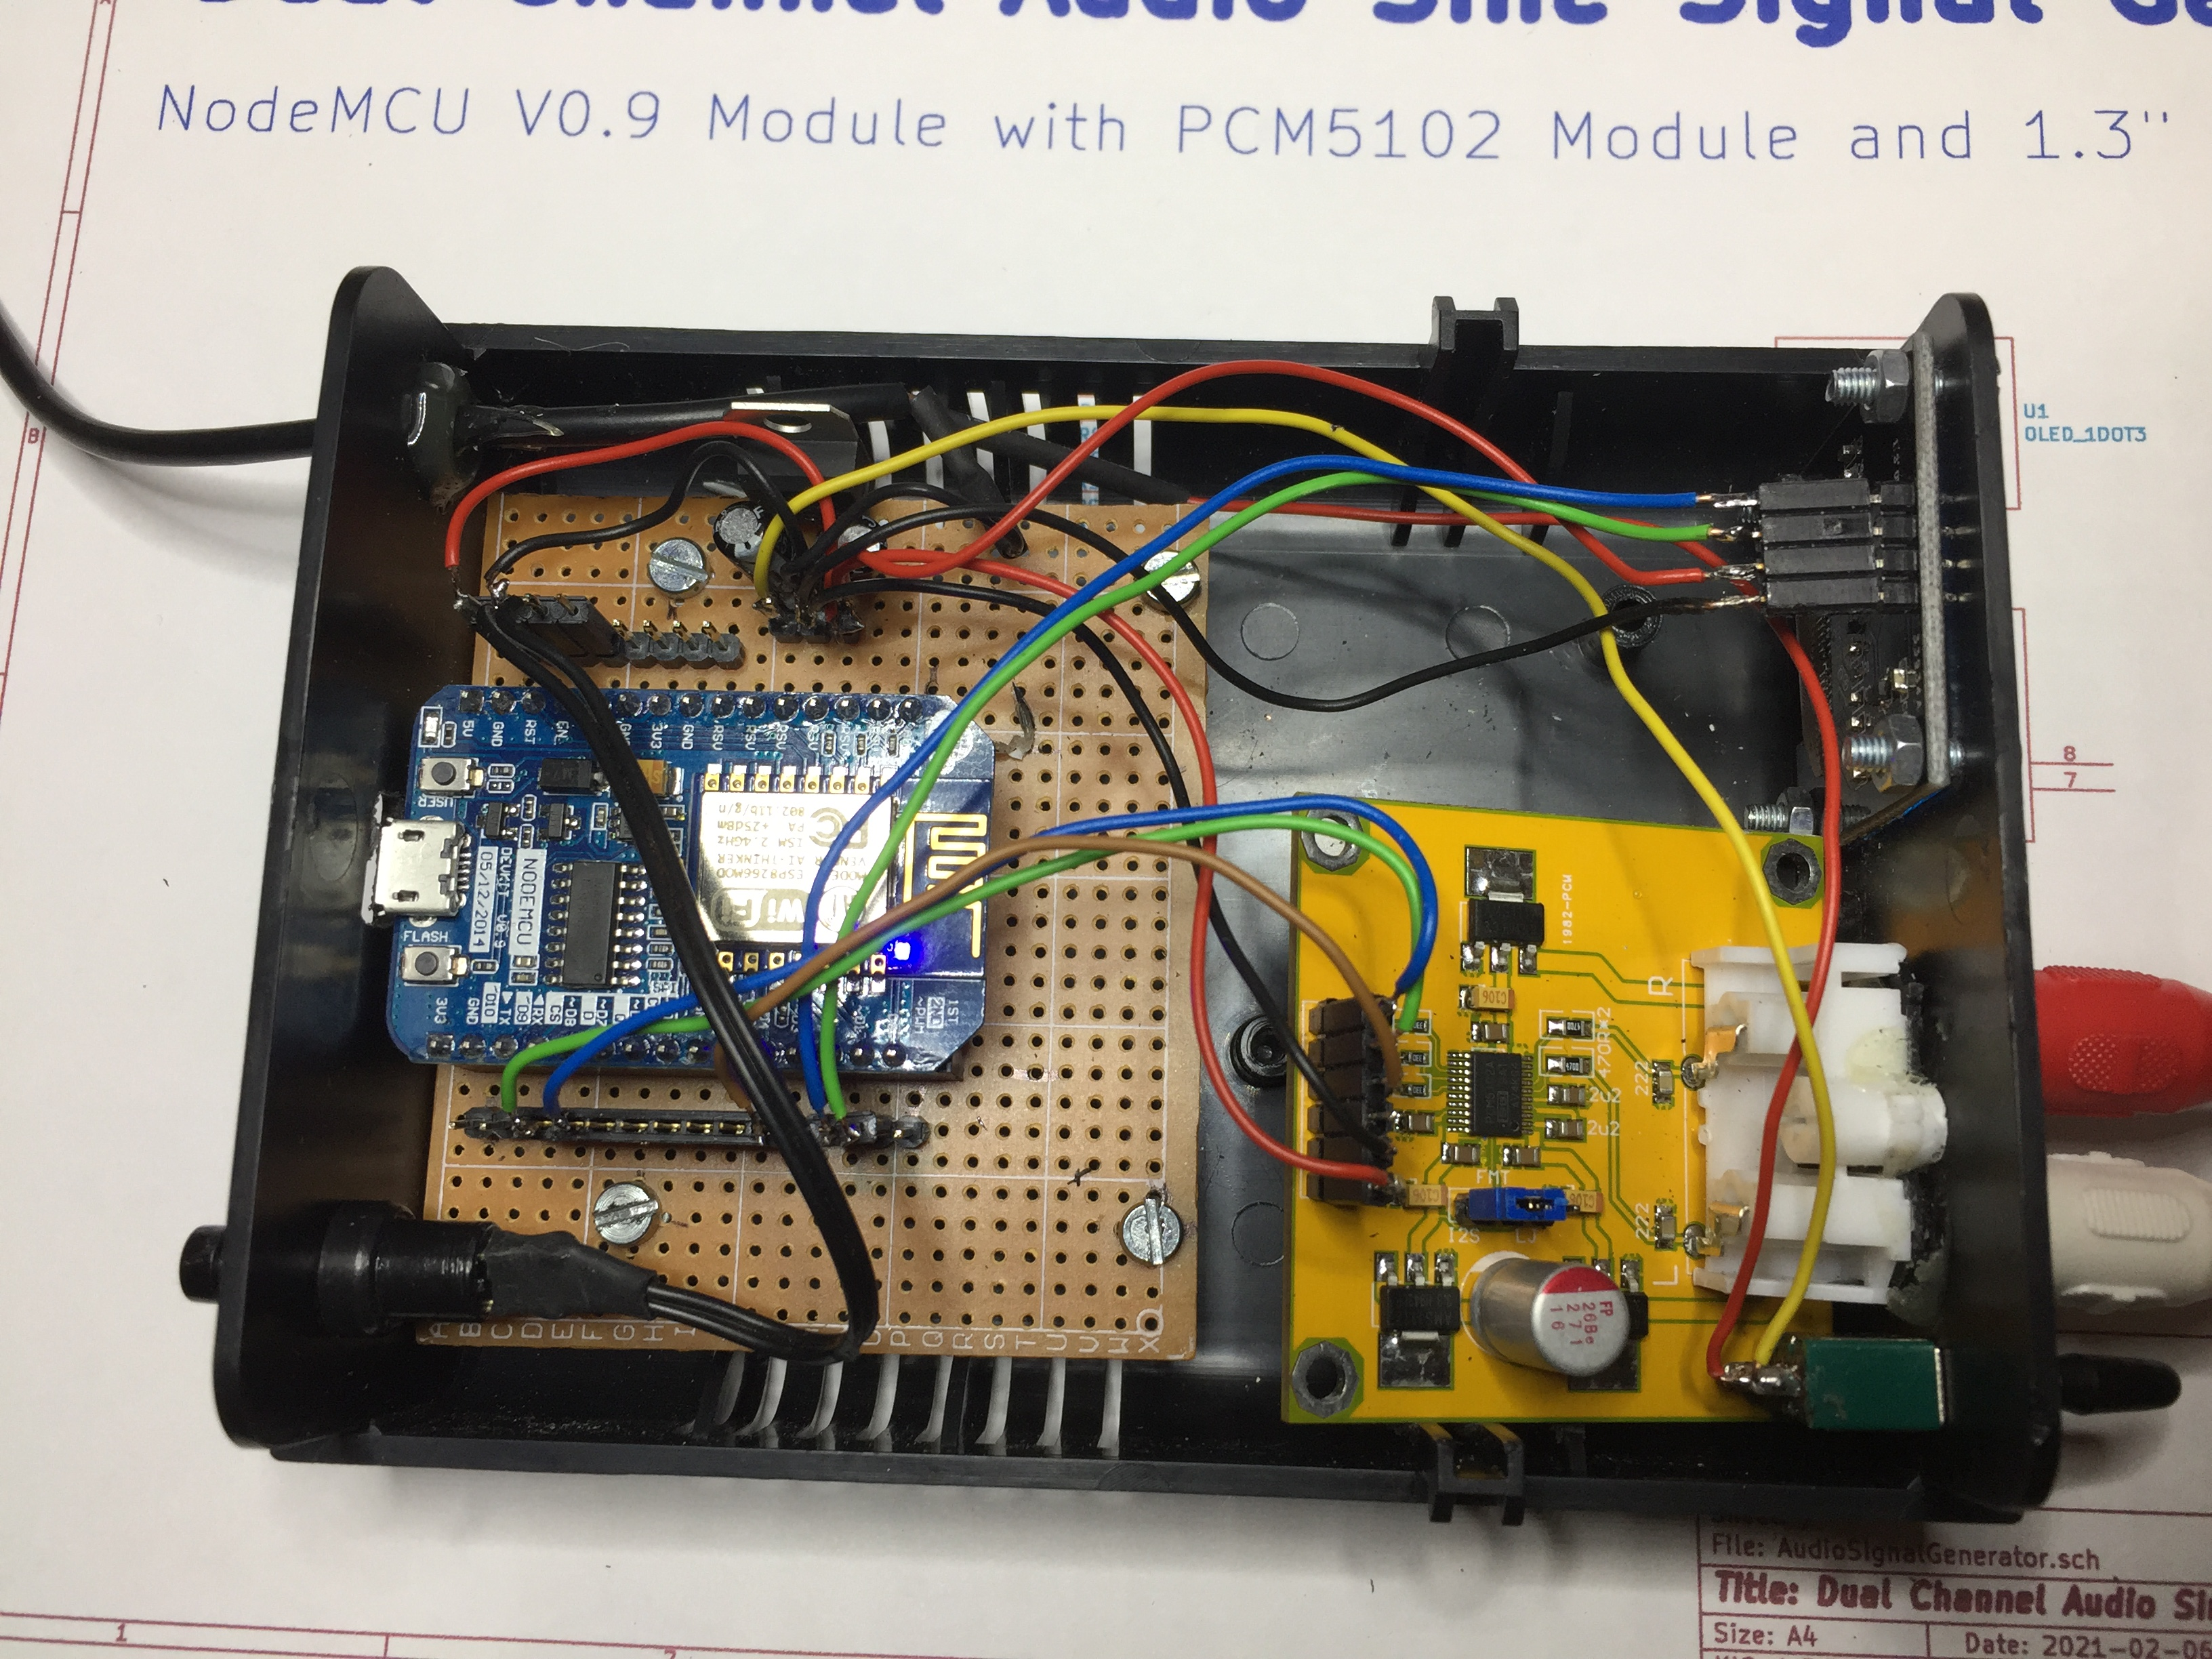
\includegraphics[width=\linewidth]{AudioSignalGeneratorTopViewOpened2.jpeg}
	\caption[Audio Signal Generator: internal mechanical assembly]{Audio Signal Generator: internal mechanical assembly}
	\label{fig:mechanics}
\end{figure}
The display is mounted on the front panel (right side in the figure). The cinch sockets of the DAC module are also going through the front panel. The on/off switch is mounted on the front panel on the left side viewed from the front.
The NodeMCU module is mounted on a bread board which also carries the power supply part. The reset button is mounted on the back panel. The power supply cable is entering the case through the back panel.
The NodeMCU is mounted inside the case such that its USB connector can be easily connected via a USB socket and cable
from the back plate. This is visible in the following back view picture of the case, showing also the reset button and the power supply cable:
\begin{figure}[tbph]
	\centering
	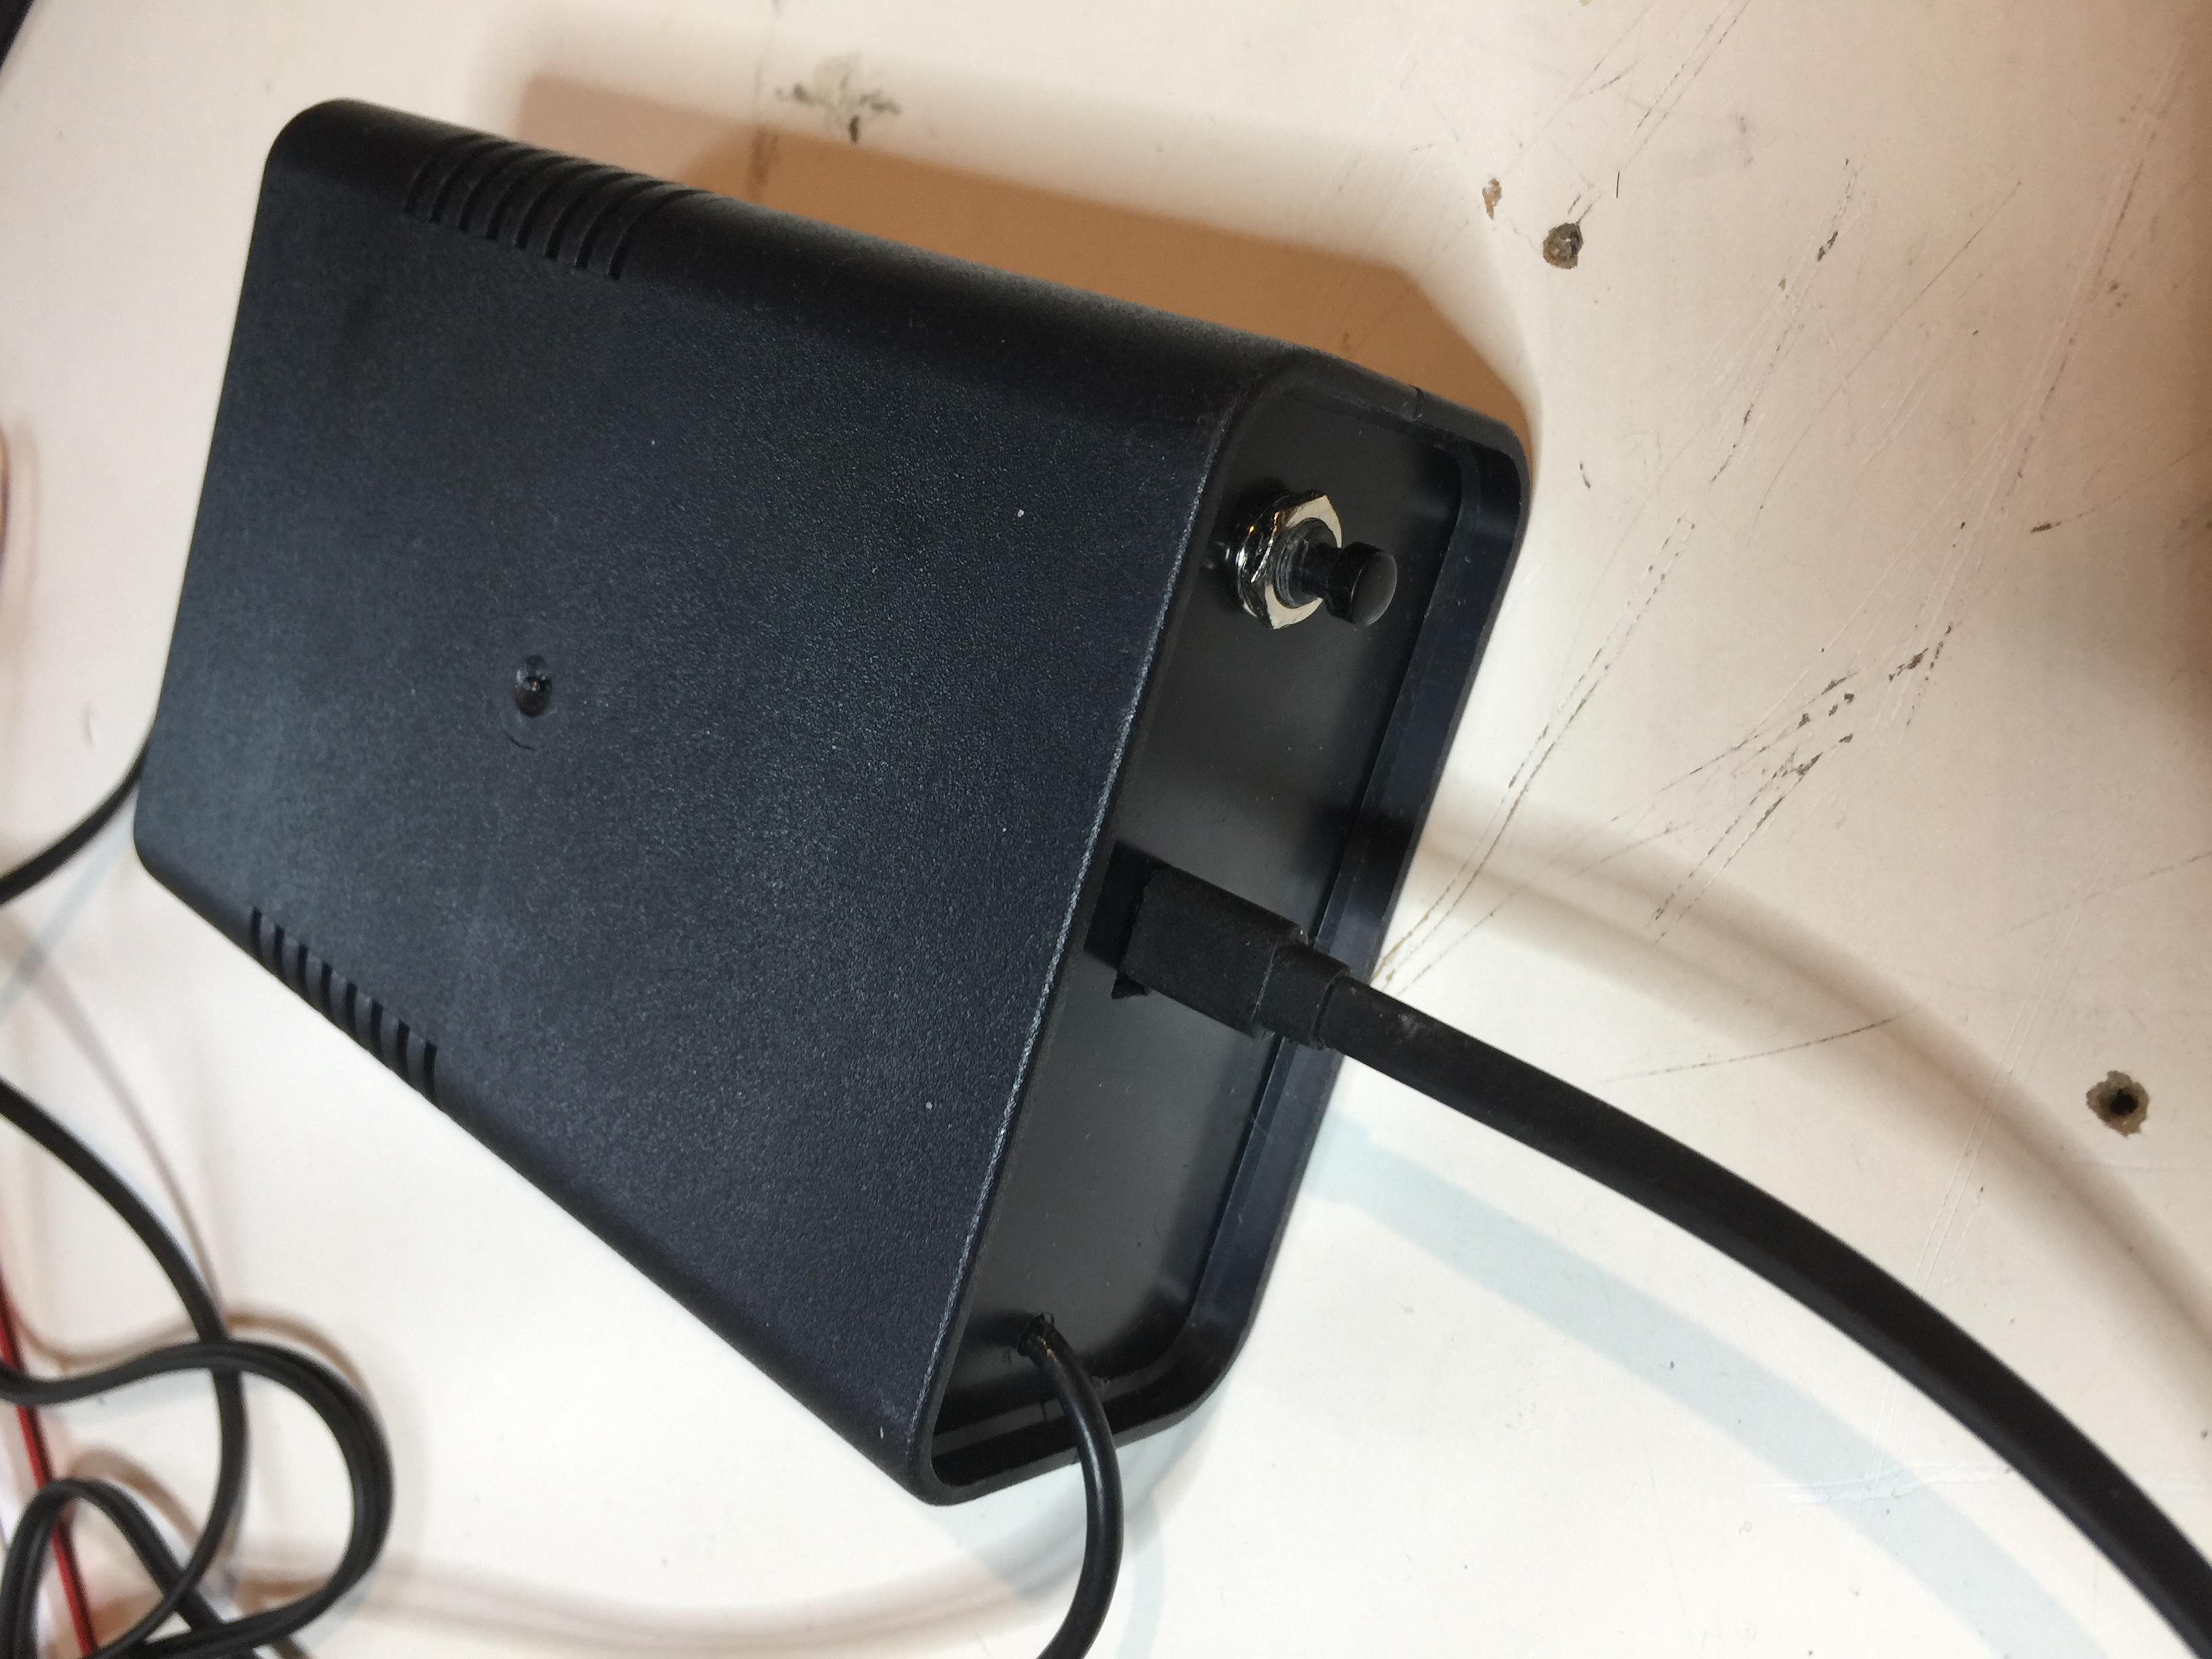
\includegraphics[width=\linewidth,angle=-90]{AudioSignalGeneratorTopBackViewClosed.jpeg}
	\caption[Audio Signal Generator: back view]{Audio Signal Generator: back view}
	\label{fig:mechanics}
\end{figure}

\newpage

\section{Schematics}
The top level schematic of the Stereo Audio Signal Generator is shown in figure \ref{fig:toplevelschematic}.
\begin{figure}[tbph]
	\centering
	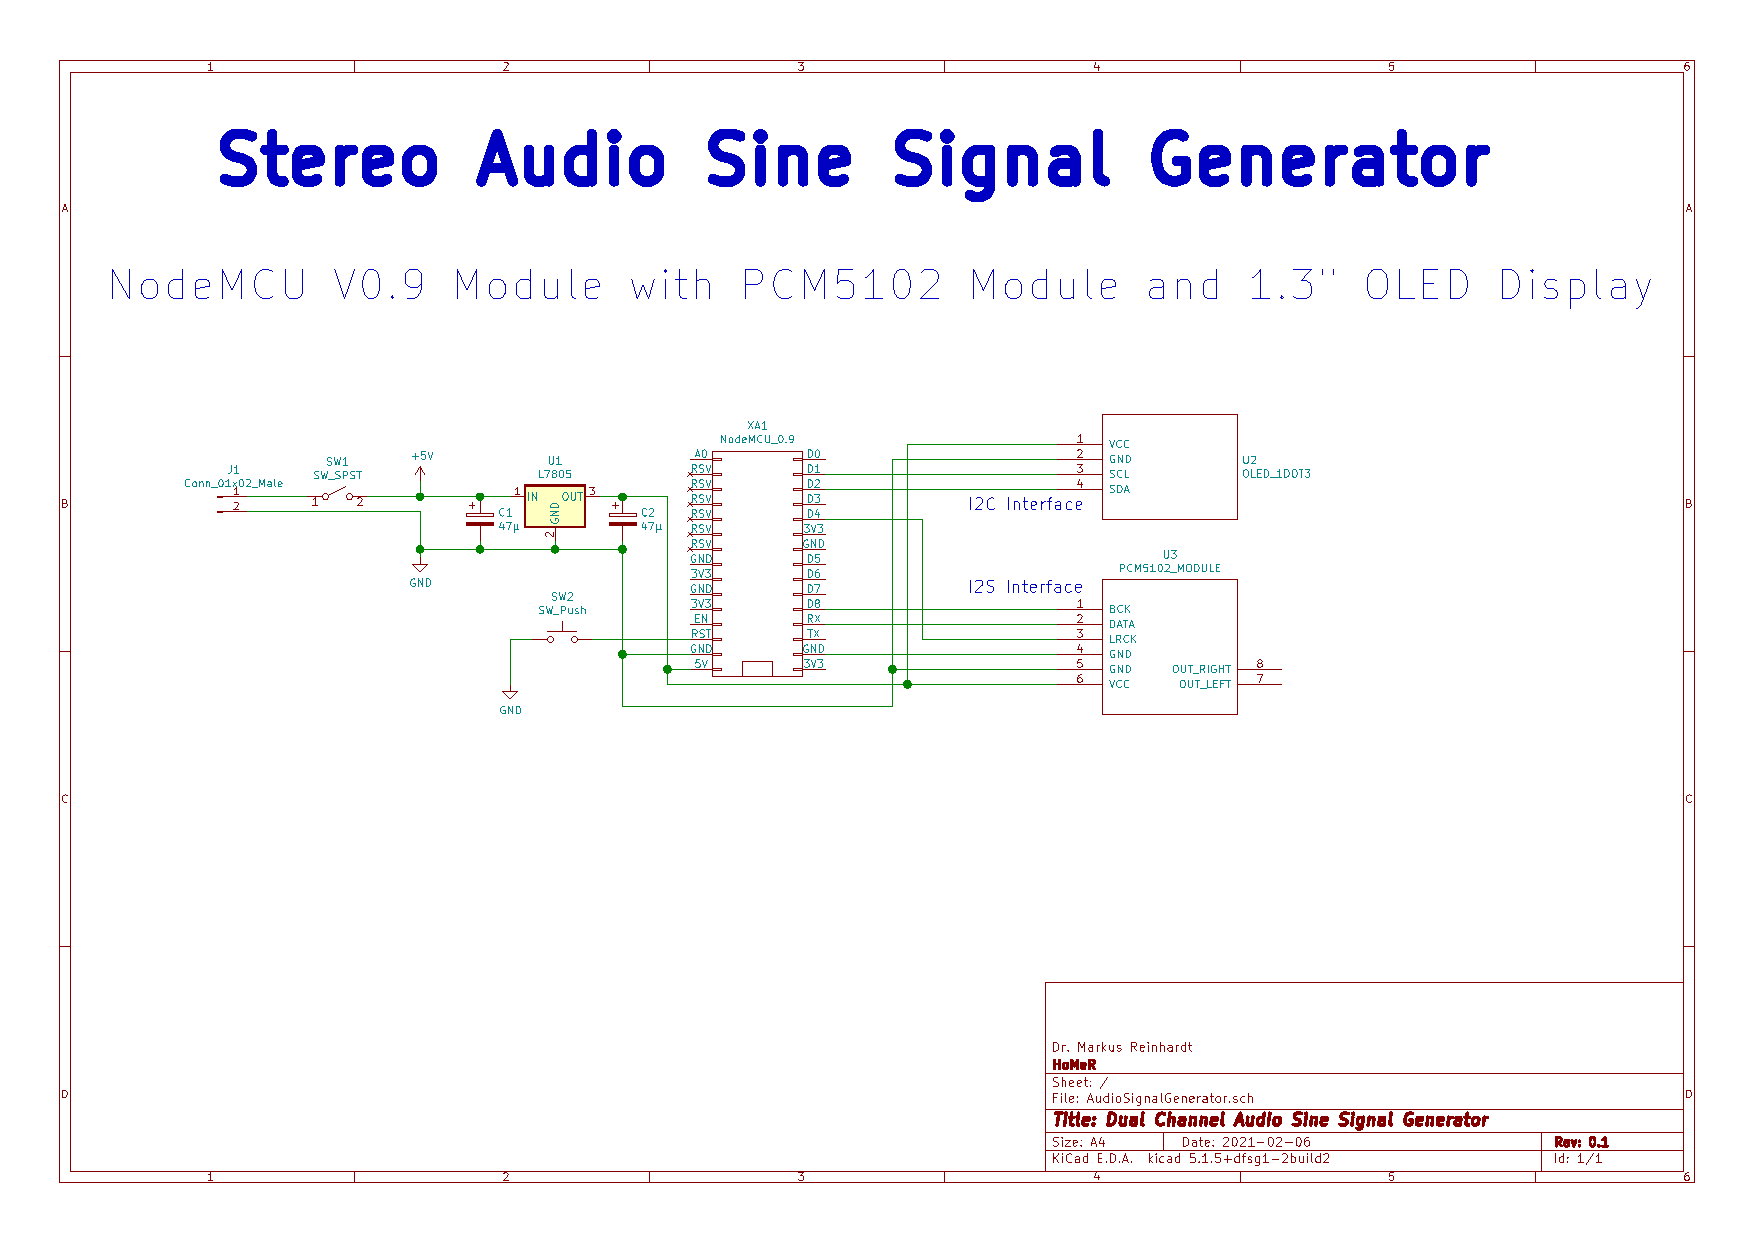
\includegraphics[width=\linewidth]{AudioSignalGeneratorSchematics.pdf}
	\caption[Audio Signal Generator top level schematics]{Audio Signal Generator top level schematics}
	\label{fig:toplevelschematic}
\end{figure}
The main controller is a NodeMCU module (V0.9) that runs the software to create I2S signals for the DAC module and the soft
ware to feed the display via the I2C interface. The DAC module is pre-built and available off-the-shelf. The 
power supply regulator is of type LM7805. Two capacitors at the input and output care for a low noise power supply voltage of 5V. The controller can be reset with a reset push-button, connecting the RST pin of the NodeMCU module to ground.
\newpage

\section{Software description}
The software is realized via the Arduino IDE and Arduino environment. The sketch is named AudioSignalGeneratorESP8266PCM5102.ino.

\subsection{Existing functionality}
The software consists mainly of two parts. The first part realizes the generation of I2S signals for stereo signals, the second part realizes the control of the display. Stereo signal generation is implemented with separate C++ classes for the signal generation itself (files ESP8266DDSGenerator.h / ESP8266DDSGenerator.cpp) and for the I2S interface handling (files IS2Handler.h / IS2Handler.cpp). The display handling is based on the U8G2 library and the routine displaySetup() called from the setup() routine of the main Arduino sketch.
In the current version the software creates the signals with a sample rate of 48kHz and each sample for the left and right channel is 16bit wide.

\subsection{Planned software extensions}
A webserver shall be implemented with the NodeMCU module such that the signal generation can be parameterized via WLAN
and a browser.

\end{document}